\subsection{\texorpdfstring{Manifold of class \(C^{r,s}\) over a manifold of class \(C^{r}\)}{Manifold of class C\^{}\{r,s\} over a manifold of class C\^{}\{r\}}}

Throughout this section, we denote by B a differentiable manifold of class \(C^{r}\) .

15.2.1. Let X be a set equipped with a map \(p: \mathbf{X} \to \mathbf{B}\) . We call a chart of X over B a triple \(\theta = (\mathbf{V}, \psi, \mathbf{F})\) , where V is a subset of X, F is a Banach space over K, and \(\psi\) is a bijection from V onto an open subset of \(\mathbf{B} \times \mathbf{F}\) such that \(\mathrm{pr}_1 \circ \psi = p|\mathbf{V}\) .

Let \((\theta_{i})_{i\in I} = ((V_{i},\psi_{i},F_{i}))_{i\in I}\) be a family of charts of X over B. We say that the \(\theta_{i}\) are \(C^{r,s}\)-compatible if, for every pair of elements \(i,j\) of I, the following two conditions are satisfied:

\begin{enumerate}
\def\labelenumi{\alph{enumi})}
\item
  \(\psi_i(V_i \cap V_j)\) is open in \(B \times F_i\) and \(\psi_j(V_i \cap V_j)\) is open in \(B \times F_j\) ;
\item
  the map \(\psi_i\circ\psi_j^{-1}\) from \(\psi_j(V_i\cap V_j)\) to \(\psi_i(V_i\cap V_j)\) is an \(\mathrm{Id}_{\mathbf{B}}\)-morphism of class \(\mathbf{C}^{r,s}\) (15.1.7).
\end{enumerate}

A family \(((\mathrm{V}_i,\psi_i,\mathrm{F}_i))_{i\in I}\) of charts of X over B that are \(\mathbf{C}^{r,s}\)-compatible and whose domains \(\mathrm{V}_i\) cover X is called a \(\mathbf{C}^{r,s}\)-atlas of X (over B). Two \(\mathbf{C}^{r,s}\)-atlases are said to be equivalent if their union is again a \(\mathbf{C}^{r,s}\)-atlas; the relation of equivalence between \(\mathbf{C}^{r,s}\)-atlases is an equivalence relation. An equivalence class of \(\mathbf{C}^{r,s}\)-atlases is called a manifold structure of class \(\mathbf{C}^{r,s}\) over B on the set X; when one wishes to specify K, one writes \(\mathbf{C}_{\mathbb{K}}^{r,s}\) instead of \(\mathbf{C}^{r,s}\) . If X is a manifold of class \(\mathbf{C}^{r,s}\) over B, we say that \(p\colon X\to B\) is the projection of X; if \(\theta\) is a chart of X over B, we say that \(\theta\) is a chart of the \(\mathbf{C}^{r,s}\)-manifold X if \(\theta\) belongs to an atlas of the equivalence class defining the structure of X.

Let X be a manifold of class \(C^{r,s}\) over B, with projection p. There exists on X

a differentiable-manifold structure of class \(\mathbf{C}^{r}\), and only one, such that, for every chart \((V,\psi,F)\) of the \(\mathbf{C}^{r,s}\)-manifold X, V is open in X and \(\psi\) is a \(\mathbf{C}^{r}\)-isomorphism of the open submanifold V of X onto the open submanifold \(\psi(V)\) of \(\mathbf{B}\times F\). If one equips X with this structure, the map \(p:X\to B\) is a submersion of class \(\mathbf{C}^{r}\) .

Let \(b \in \mathbf{B}\) and let \(\mathbf{X}_b = p^{-1}(b)\). There exists a K-manifold structure of class \(\mathbf{C}^s\) on \(\mathbf{X}_b\), and only one, such that, for every chart \(\theta = (\mathbf{V}, \psi, \mathbf{F})\) of the \(\mathbf{C}^{r,s}\)-manifold \(\mathbf{X}\), the triple \(\theta_b = (\mathbf{V} \cap \mathbf{X}_b, \operatorname{pr}_2 \circ \psi | (\mathbf{V} \cap \mathbf{X}_b), \mathbf{F})\) is a chart of the manifold \(\mathbf{X}_b\). The differentiable-manifold structure of class \(\mathbf{C}^r\) underlying this structure is induced by the differentiable-manifold structure of class \(\mathbf{C}^r\) on \(\mathbf{X}\) defined above.
% semantic-fragments: legacy-input-seam
\relax{}
15.2.3. Examples

\begin{enumerate}
\def\labelenumi{(\roman{enumi})}
\item
  When B is reduced to a point, the notion of a manifold of class \(C_{K}^{r,s}\) over B is equivalent to that of a K-manifold of class \(C^{s}\) .
\item
  Let Z be a K-manifold of class \(C^{s}\) ; take \(X = B \times Z\) and \(p = pr_{1}\) . There exists on X a structure of manifold of class \(C^{r,s}\) over B, and only one such structure, such that, for every chart \((U, \psi, L)\) of Z, \((B \times U, Id_{B} \times \psi, L)\) is a chart of the \(C^{r,s}\) -manifold X.
\item
  Let X be a manifold of class \(C^{r,s}\) over B, and let Y be an open subset of X. The structure of manifold of class \(C^{r,s}\) of Y induced by that of X is defined as in the case of manifolds (cf.~5.2.3).
\item
  Let M be a vector bundle over K with base B and of class \(C^{r}\) (7.3.4), and let \(\pi\) be its projection onto B. There exists on M a structure of manifold of class \(C_{K}^{r,\omega}\) over B, and only one, such that, if \((\mathbf{U},\psi,\mathbf{F})\) is a K-vector chart of M (8.8.1), the triple \((\pi^{-1}(\mathbf{U}),\psi,\mathbf{F})\) is a chart of the \(C_{K}^{r,\omega}\) -manifold M.
\end{enumerate}

15.2.4. Let X be a manifold of class \(C^{r,s}\) over B, p its projection, L a K-Banach space, and f a mapping of X into L. We say that f is of class \(C^{r,s}\) if, for every chart (V, \(\psi\) , F) of the \(C^{r,s}\) -manifold X, the mapping ( \(f|V) \circ \psi^{-1}\) of \(\psi(V)\) into L is of class \(C^{r,s}\) (15.1.6). Such a mapping is of class \(C^{r}\) and its restriction to \(X_{b}\) for \(b \in B\) , is of class \(C^{s}\) .

15.2.5. Let \(g: \mathbf{B} \to \mathbf{B}'\) be a morphism of differentiable manifolds of class \(\mathbf{C}^{r}\) and let

\pandocbounded{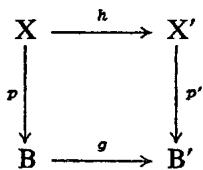
\includegraphics[keepaspectratio]{images/part001_9e08a31f.jpg}}

X (resp. X') be a manifold of class \(C^{r,s}\) over B (resp. B'), and let h be a mapping from X into X'. We say that h is a g-morphism of class \(C^{r,s}\) if the following three conditions are satisfied:

\begin{enumerate}
\def\labelenumi{\alph{enumi})}
\item
  \(p^{\prime}\circ h = g\circ p;\)
\item
  h is continuous;
\item
  for every chart \((\mathrm{V}^{\prime},\psi^{\prime},\mathrm{F}^{\prime})\) of the \(C^{r,s}\) -manifold \(X^{\prime}\) , the map \(pr_{2}\circ\psi^{\prime}\circ h\) of \(V=h^{-1}(V^{\prime})\) to \(F^{\prime}\) is of
\end{enumerate}

class \(\mathbf{C}^{r,s}\) (in the sense of 15.2.4) when one endows the open set V with the structure induced by that of X (15.2.3, (iii)).

When \(\mathbf{B} = \mathbf{B}'\) and \(g = \mathrm{Id}_{\mathbf{B}}\) , we also say that \(h\) is a B-morphism of class \(\mathbf{C}^{r,s}\) .

For a B-morphism of class \(C^{r,s}\) to be a B-isomorphism of class \(C^{r,s}\) , it suffices that it be an isomorphism of class \(C^{1}\) .

Let \(g': B' \to B''\) be a morphism of manifolds of class \(C^r\) and let \(X''\) be a manifold of class \(C^{r,s}\) over \(B''\) . If \(h: X \to X'\) is a \(g\) -morphism of class \(C^{r,s}\) and \(h': X' \to X''\) is a \(g'\) -morphism of class \(C^{r,s}\) , then \(h' \circ h\) is a \((g' \circ g)\) -morphism of class \(C^{r,s}\) .

15.2.6. Let X be a manifold of class \(\mathbf{C}_{\mathbf{R}}^{r,s}\) over B and \(p\) its projection; we assume \(s \neq \omega\) , X is separated, and \(p\) is proper (TG, I, § 10, no. 1). Then, for every \(b \in \mathbf{B}\) there exists an open neighborhood U of \(b\) and a \(\mathbf{C}^{r,s}\) -isomorphism from \(p^{-1}(\mathbf{U})\) onto \(\mathbf{U} \times \mathbf{X}_b\) , where \(\mathbf{X}_b = p^{-1}(b)\) .

15.2.7. Let X be a manifold of class \(C_{K}^{r,s}\) over B, p its projection, and \(\sigma: B \to X\) be a section of class \(C^{r}\) . We call a tubular neighborhood of class \(C_{K}^{r,s}\) of \(\sigma\) a triple (M, N, \(\varphi\) ) where M is a K-vector bundle, with base B and of class \(C^{r}\) , N is an open neighborhood of \(\sigma(\mathbf{B})\) in X, and \(\varphi\) is a B-isomorphism of class \(C_{K}^{r,s}\) from N onto an open subset of M (cf. 15.2.3 (iv)), mapping the section \(\sigma\) to the zero section of M.

Suppose that \(s \geqslant r + 1\) and that the manifold B is paracompact and admits partitions of unity of class \(\mathbf{C}^{r}\) (5.3.6); there then exist tubular neighborhoods of class \(\mathbf{C}_{\mathbb{K}}^{r,s}\) of \(\sigma\) .

